\section{Practicality of Covert Communication}
\label{sec:study}

In this section, we present an evaluation on the practicality of a lambda covert
channel that is discovered with our co-residence detector.  The amount of
information that can be transferred depends on two factors: 1) the channel
capacity and 1) the number of co-resident clusters of lambdas, or rendezvous
points, that materialize during the attack.  We first produce an estimate on the
capacity of the covert channels established, and then examine the co-residence
density in various AWS regions to understand the number of rendezvous points and
factors that affect it.

\subsection{Covert Channel Capacity}

\begin{figure}[!t]
  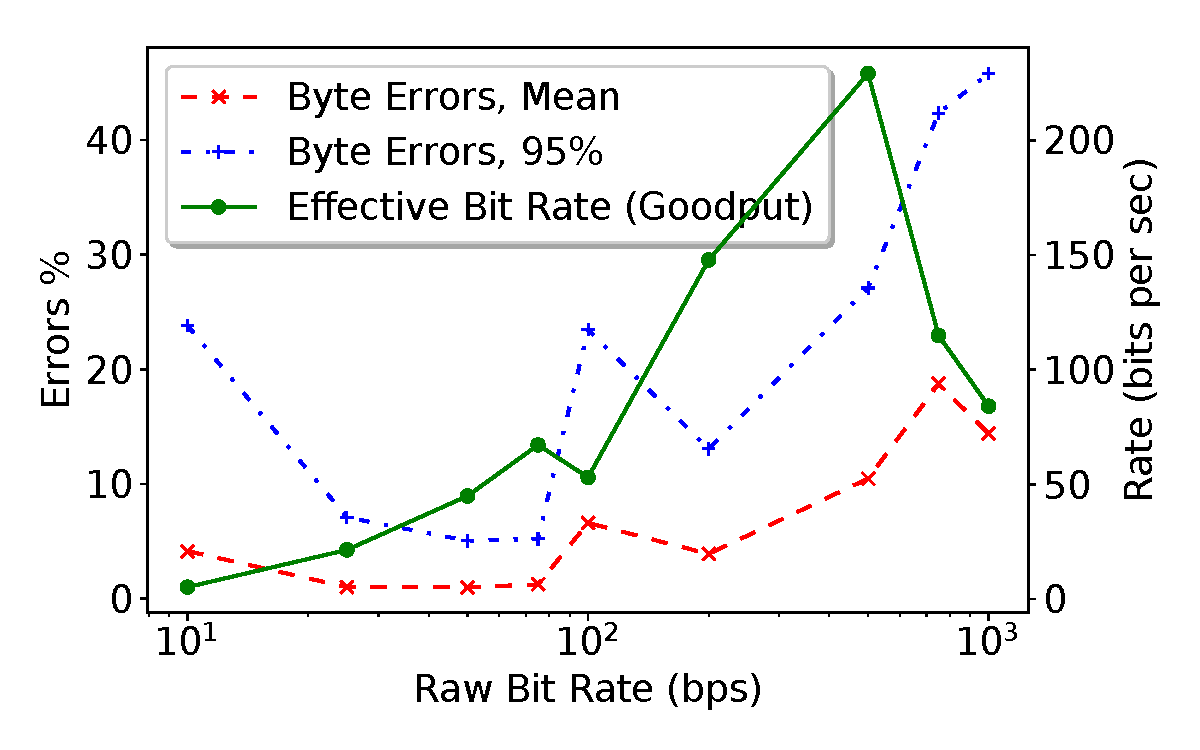
\includegraphics[width=.99\linewidth]{fig/channel_rate_3gb.pdf}
  \caption{\todo{increase font}
\label{fig:channel}}
\end{figure}

Once co-residence between any two lambas is established, the attacker can then
use the same memory bus hardware to perform covert communication. Wu et
al.~\cite{wuusenix2012}, who first introduced covert channel based on this
hardware channel, also presented an efficient and error-free communication
protocol targeting cloud-based platforms like VMs.  While such a protocol should
theoretically work for lambdas, extending it is beyond the scope of this work.
We do, however, use a much simpler (albeit more inefficient) protocol to report
a conservative estimae of the capacity of each covert channel.

Our protocol for data transfer uses the same mechanisms used for co-residence
detection in section \todo{ref 5.2} to send and receive bits and perform clock
synchronization. However, since we can use our co-residence detector to identify
lambdas on a machine and target the two that we wish to label as the sender and
receiver, we are not concerened about noise from multiple receivers, and as such
can allow the receiver to sample continuously (\todo{ref}) and sample at
extremely small intervalls (milliseconds instead of seconds). While we want the
sampling interval to be as small as possible (in order to increase the rate of
bits transferred), the chances of erasures or errors also increases as the
sender and receiver may get descheduled during this time. 

To demonstrate this, we launched hundreds of 3 GB lambdas on AWS and use our
co-residence detector to establish tens of covert channels. We then send data
over these channels at various bitrates and record the error ratio (for
byte-sized data segments). Figure~\ref{fig:channel} shows the mean error ratio
at 50\% and 95\% confidence intervals, both of which increase with the bitrate.

%The only difference is that since we now only expect just the
%sender and receiver lambdas to be active (i.e., although there may be tens of
%other co-resident lambdas, we can use our co-residence detector to identify
%every lambda and set others inactive), we don't need to worry about noise from
%multiple receivers, the result being receiver can sample continously (\todo{ref
%5.2.2}) and time spent for each bit can be extremely small (in the order of
%milliseconds instead of seconds). 
%Naturally, we want this time to be as small as possible to increase bitrate,
%however, the chances of erasures (errors) increase too as both sender and
%receiver may get descheduled during this time.  
%To demonstrate this, we launch
%hundreds of (3 GB) lambdas on AWS and use our co-residence detector to establish
%tens of covert channels. We then send data over these channels at various
%bitrates and record the error ratio (for byte-sized data segments).
%Figure~\ref{fig:channel} shows the mean error ratio at 50\% and 95\% confidence,
%both of which increase with the bitrate.

To correct these errors, we can use block-based error correction codes like
Reed-Solomon, which uses byte-sized encoded symbols~\cite{wuusenix2012} as
descheduling may result in burst errors\amirian{do we need to define this? is this
important?}.
However, error correction comes with an overhead; Reed-Solomon requires twice as
many extra symbols\amirian{why dont we just use the term bytes here instead of
symbols?} as there are errors to correct. So, for each bitrate, we must compute
effective bitrate by subtracting the overhead of error correction symbols.
%required to correct its corresponding 95\% error. 
From Figure~\ref{fig:channel}, we can see that effective bitrate rises to a
maximum of over 200 bits per second (bps) (at 500bps raw rate) before falling
again due to high error rate. We confirmed this by sending Reed-Solomon encoded
data over the covert channels at this rate and observed near-zero data
corruption. Thus, we conclude that, by a conservative estimate, we can safely
send data across each of these covert channels at a rate of ~200 bps.

\subsection{Rendezvous point density}
\todo{Changes due to above subsection}
Next, we present measurements on serverless function density on AWS using our
co-residence detector, and discuss the factors that may affect this density.  As
we discussed earlier, the key challenge in enabling traditional covert channels
on the cloud is identifying which lambdas are on the same machine. We attempt to
answer the following question: assuming that the user launches a number of
(sender and receiver) lambdas at a specific point in time, what is the expected
number of such co-resident pairs that they might see? We deploy a large number
of lambdas on various AWS regions and report the co-residence density, that is,
the average number of lambdas that end up co-resident on each servern in
figure\todo. The higher the co-residence density, the easier it is for the user
to ultimately establish covert channels with lambdas, and the more information
they can send. Unless specified otherwise, all the experiments discussed in this
section are performed with 1.5 GB lambdas and executed successfully with
\textbf{zero error} in co-residence detection.


\begin{figure*}[!t]
    \begin{subfigure}{.5\textwidth}
      \centering
      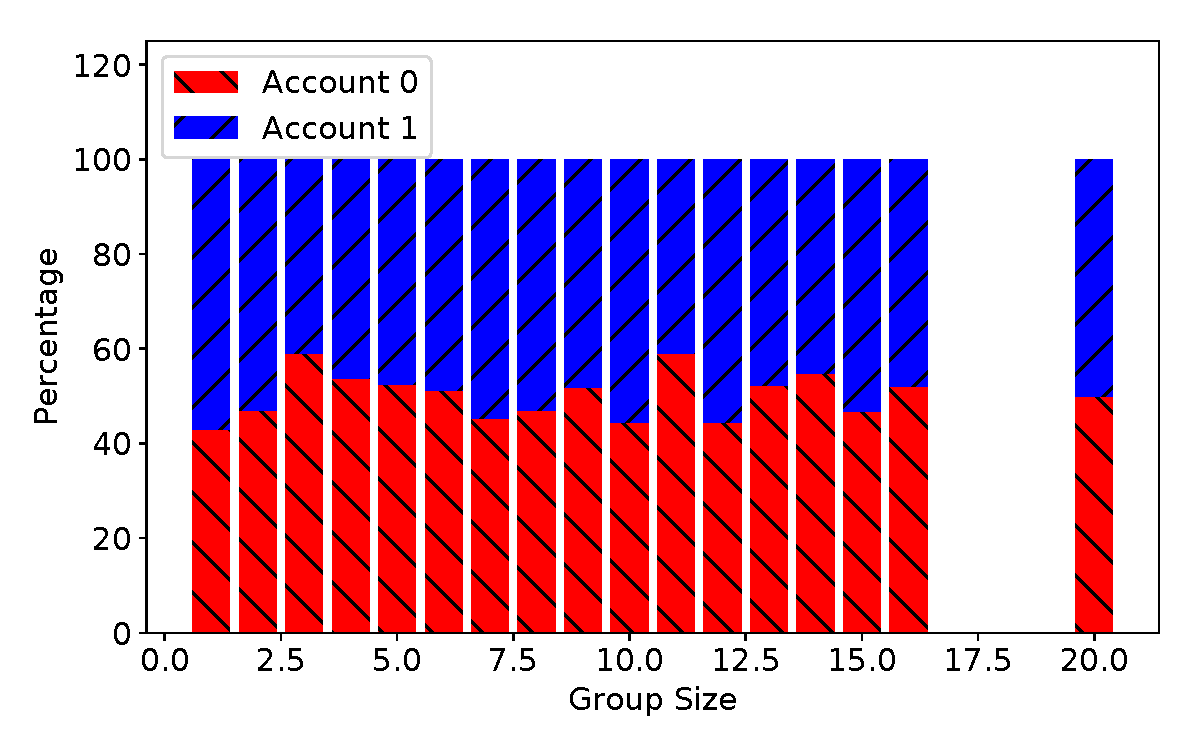
\includegraphics[width=.99\linewidth]{fig/different-accounts.pdf}
    %   \caption{1a}
    %   \label{fig:sfig1}
    \end{subfigure}%
    \begin{subfigure}{.5\textwidth}
      \centering
      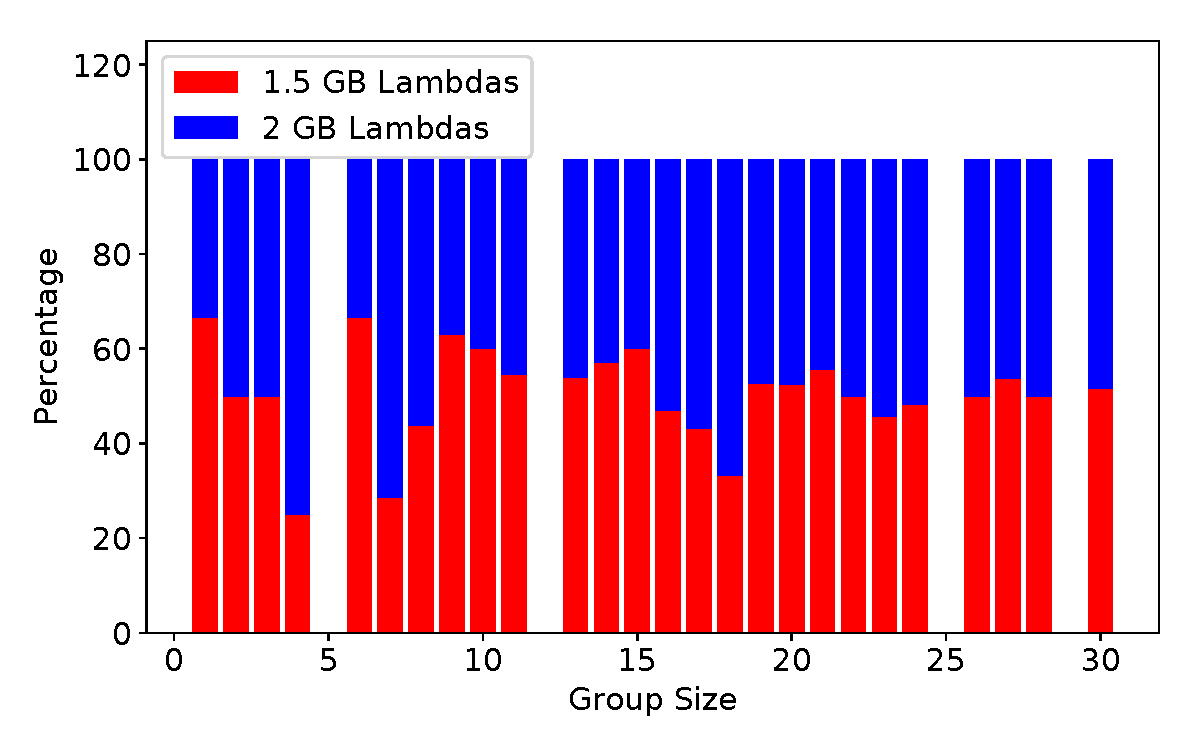
\includegraphics[width=.99\linewidth]{fig/different-sizes.pdf}
    %   \caption{1b}
    %   \label{fig:sfig2}
    \end{subfigure}

    \caption{The left plot shows the breakdown of co-resident groups (of varying
    sizes) of lambdas by two different accounts in an experiment of 1000
    lambdas, where 500 lambdas are launched from each account. The uniformity of
    the split indicates that the lambda scheduler might be invariant to the
    account the lambdas are launched from. Similar results are shown for
    different lambda sizes in the right plot. }
    \label{fig:factors}
\end{figure*}


\subsubsection{Across AWS regions}
\amirian{does this make sense here as a subsubsection?}
\todo{clarify the attacker model here, per R1 comments}
We execute our co-residence detector with 1000 1.5 GB Lambdas in various AWS
regions. Figure~\ref{fig:awsregions} comprises multiple plots depicting
the co-resident groups per region, with each bar indicating the fraction of
lambdas that detected a certain number of neighbors (i.e., that belong to a
co-resident group of a certain size). Plots that skew to the right indicate a
higher co-residence density when compared to the plots skewed to the left (also
illustrated in Figure~\ref{fig:density}). We note that, in most regions, almost
all lambdas recognize at least one neighbor (indicated by smaller or
non-existent first bar in each plot). We hypothesize that the co-residence
density is (inversely) dependent on the total number of servers and the lambda
activity in the region, both of which can be assumed to be lower in newer AWS
regions, hence the higher co-residence density in those regions as we can see in
Figure~\ref{fig:density}. The ample co-residence in general across all the
regions shows that lambdas provide a fertile ground for covert channel attacks.
%We note that the largest co-resident group on a single machine was comprised of 25 lambdas. 


\subsubsection{Other factors}
We also examine how co-residence is affected by various launch strategies that
the user may use, like deploying lambdas from multiple AWS accounts and
different lambda sizes. In particular, we wish to determine if we our mechanism
exhibits different results when: 1) the user deploys sender lambdas and receiver
lambdas on two separate accounts (normally the case with covert channels) and 2)
the senders and receivers are created with different lambdas sizes.  To answer
these questions, we run an experiment with 1000 lambdas of which we launch 500
lambdas from one account (senders) and 500 from other deployed in a random
order. The co-residence observed was comparable to the case where all the
lambdas were launched from one account. In the left subfigure of
Figure~\ref{fig:factors}, we show the breakdown of co-resident group of lambdas
of each size among the two accounts.  We can see that among the co-resident
groups of all sizes, roughly half of lambdas came from either account. This show
that lambda scheduler is agnostic to the accounts the lambdas were launched
from. We see similar results for different lambda sizes, as shown in the right
subfigure of Figure~\ref{fig:factors}.

%From our experiments, we also observe that co-residence density in a region
%barely changes during course of the day or the week (data not shown
%in any figure \todo{is this okay?}).  This gives the user the freedom to utilize this
%technique at any time and expect similar results.
